\subsection{Results}
This section presents the detected and manually-measured solidification
velocity results for each
of the two type of experiments outlined in the previous section.

% -------------------------------------------------------------------------
\subsubsection{Simulated AM Results}
% -------------------------------------------------------------------------
The simulated AM S-L interface detection procedure and manual measurement
was applied to three separate experiments to test the performance of the
procedure.
Each experiment utilized a
different laser power to melt the sample: 104 W (20\% maximum power),
156 W (30\% maximum power), and 208 W (40\% maximum power).
In the 104 W experiment, the average velocity of the three
manually identified interfaces were calculated to be 0.058, 0.056, and 0.058
m s\textsuperscript{-1} , for a collective average velocity of 0.057
m s\textsuperscript{-1} and median of 0.057 m s\textsuperscript{-1}. The
average velocity of the detected interfaces was 0.021 m s\textsuperscript{-1},
with a median of 0.041 m s\textsuperscript{-1}.

\begin{figure}[ht]
    \centering
    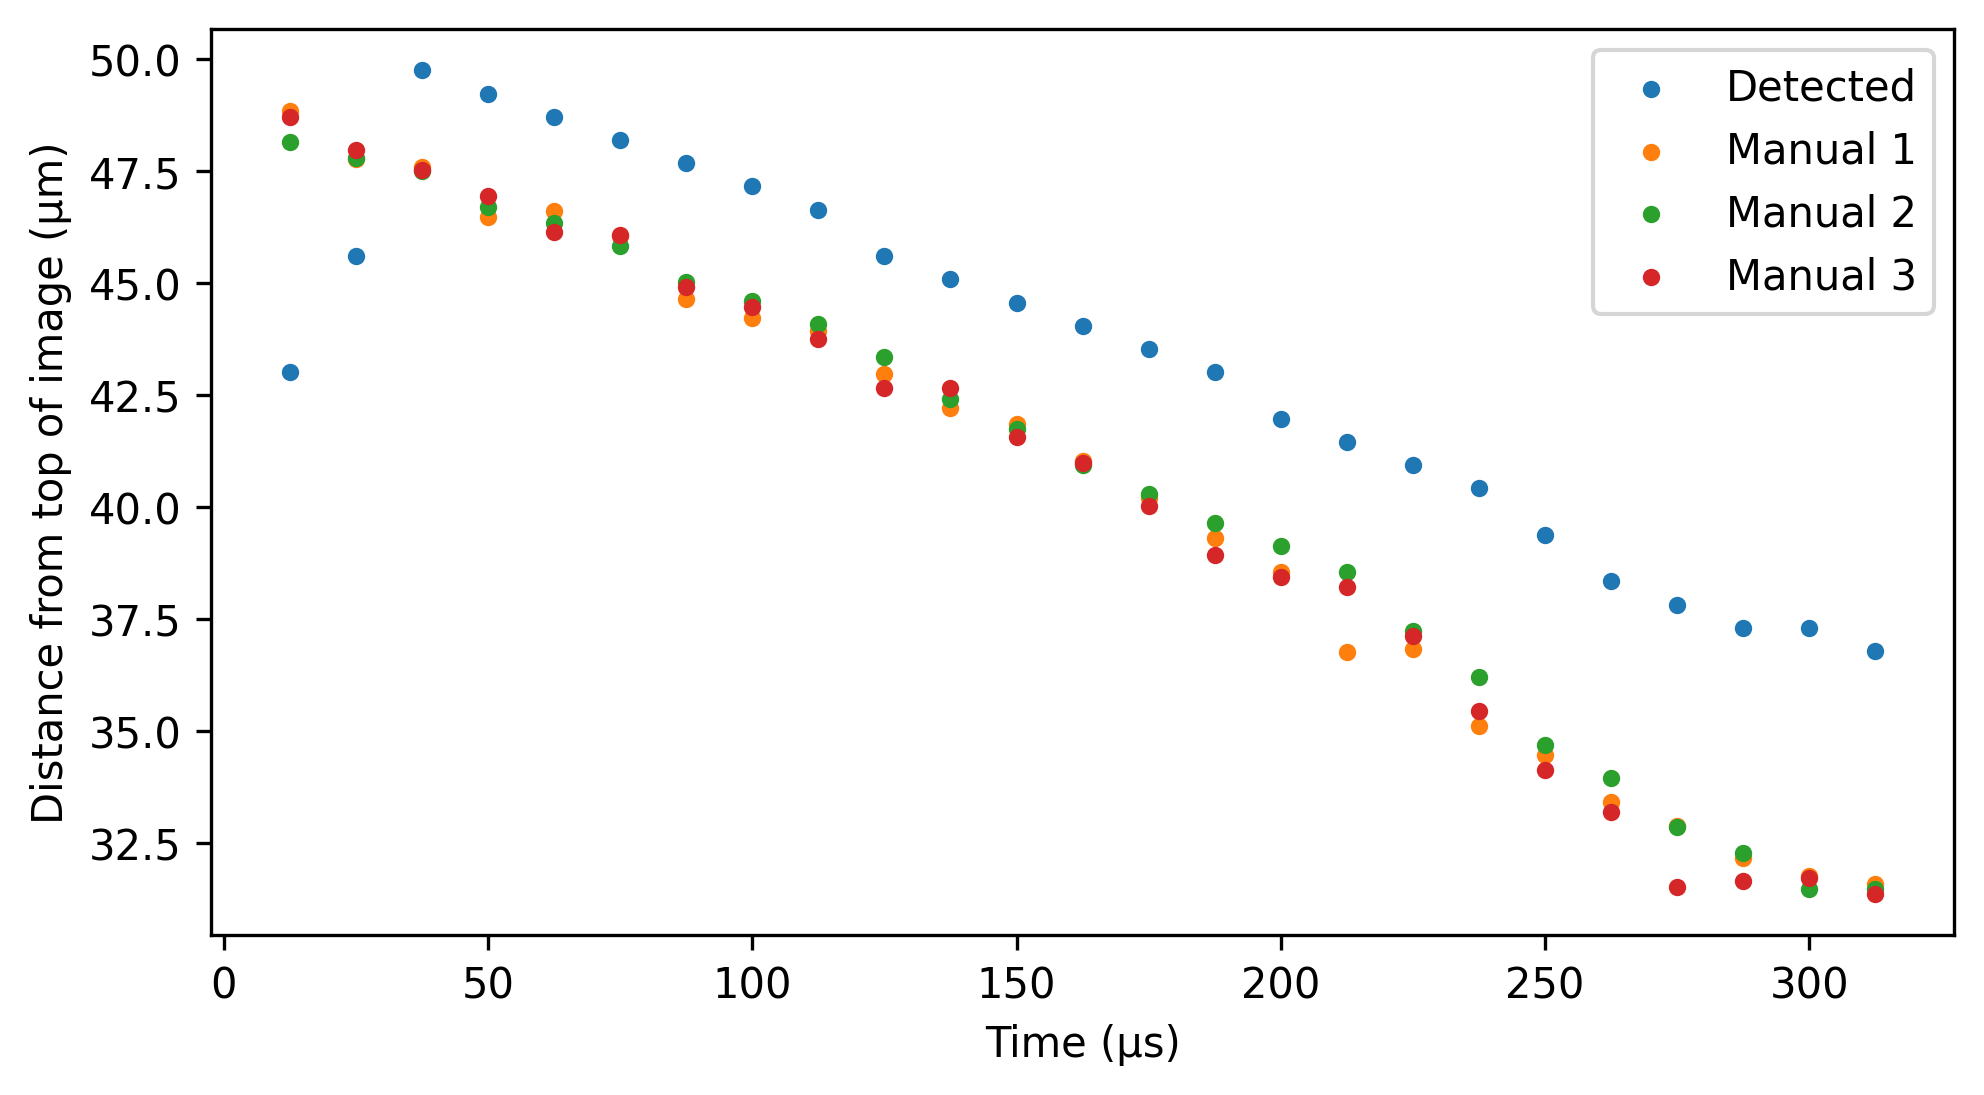
\includegraphics[width=0.75\textwidth]{figures/04/12-detected-vs-manual-1-10_shot05.png}
    \caption{
        \small\setstretch{1}
        Interfaces detected by the automated procedure (blue) compared with
        manually identified interfaces (orange, green, and red) for the
        104 W experiment. Interface location is defined by the distance from
        the bottom of the solid-liquid interface to top of the image,
        starting when the laser shuts off (t = 0 µs).
    }
    \label{fig/detected-aps-1}
\end{figure}

In the 156 W experiment, the average velocity of the three
manually identified interfaces were calculated to be 0.046, 0.046, and 0.045
m s\textsuperscript{-1}, for a collective average velocity of 0.046
m s\textsuperscript{-1} and median of 0.043 m s\textsuperscript{-1}. The
average velocity of the detected interfaces was 0.022 m s\textsuperscript{-1},
with a median of 0.041 m s\textsuperscript{-1}.

\begin{figure}[ht]
    \centering
    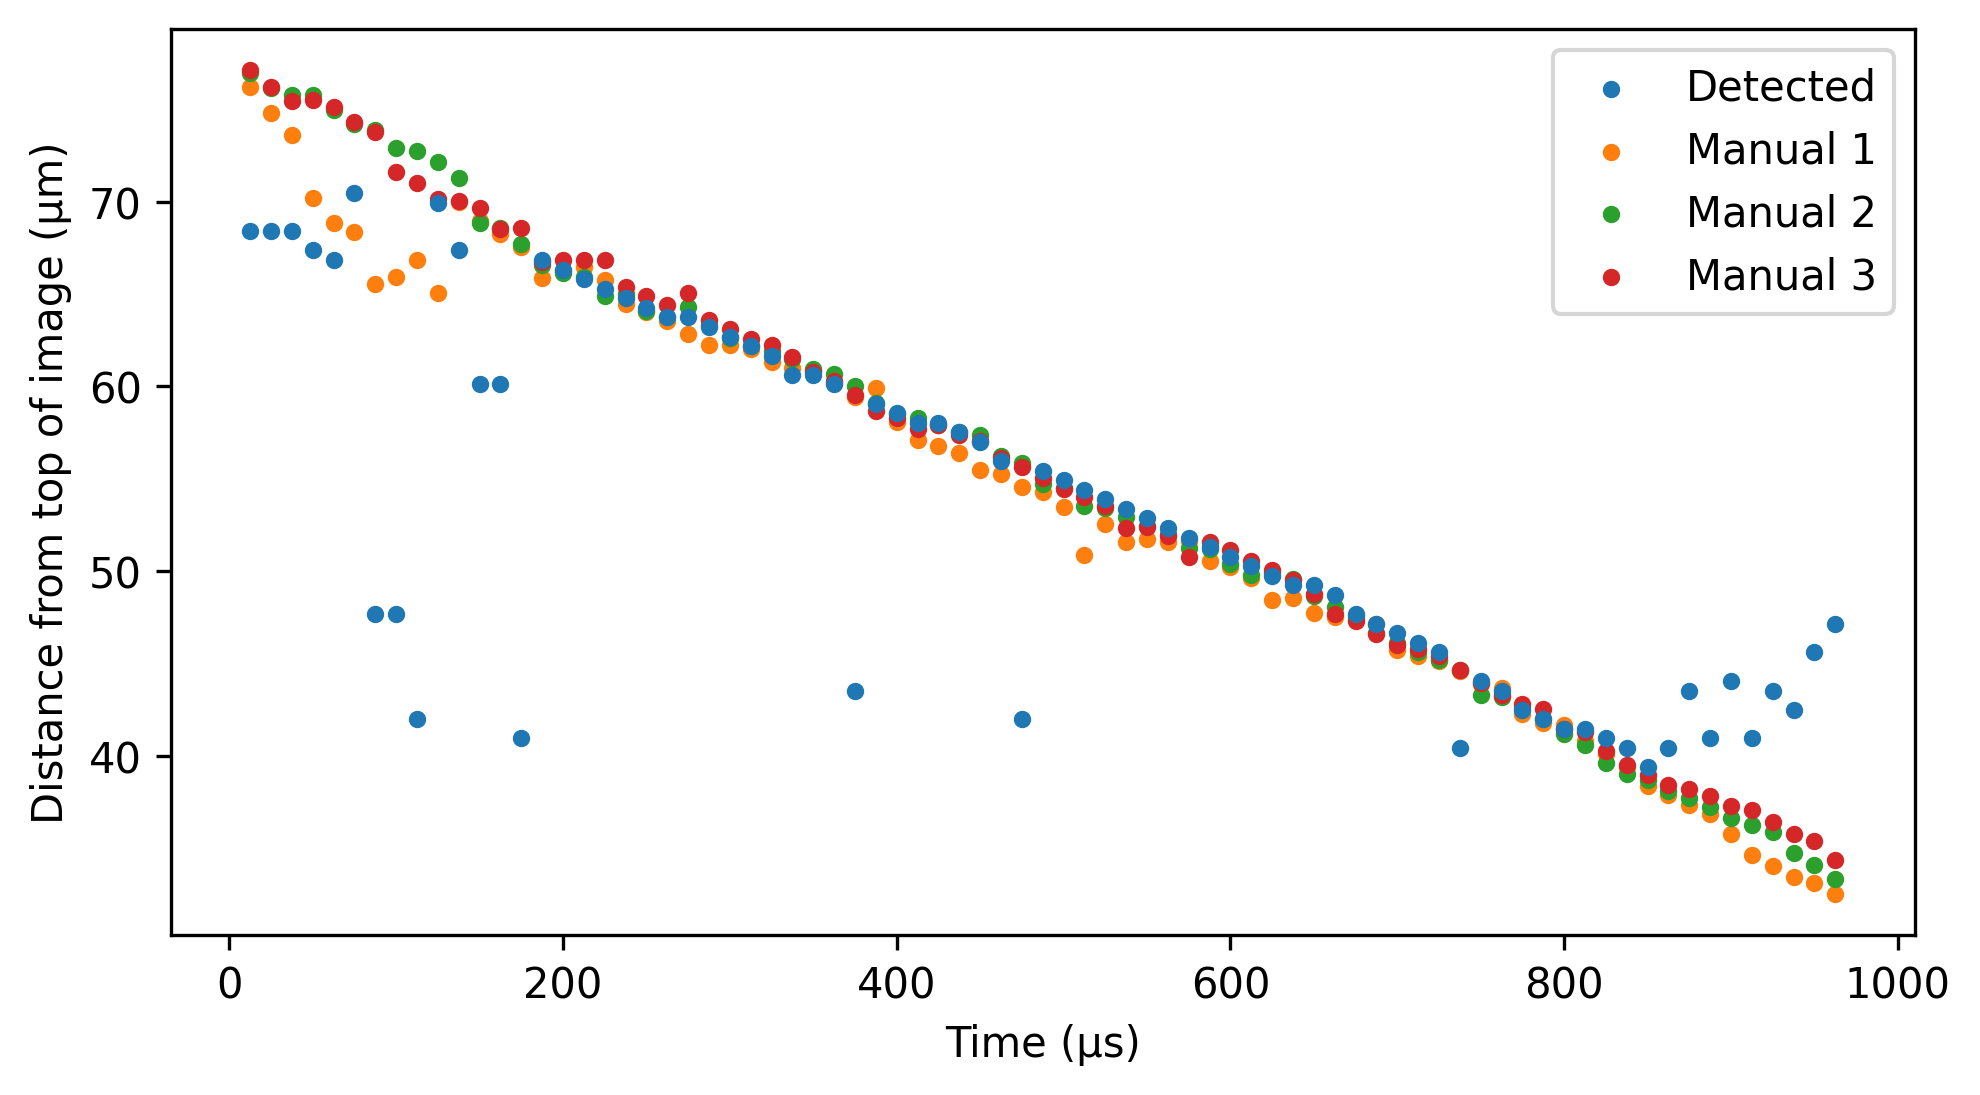
\includegraphics[width=0.75\textwidth]{figures/04/13-detected-vs-manual-2-06_shot01.png}
    \caption{
        \small\setstretch{1}
        Interfaces detected by the automated procedure (blue) compared with
        manually identified interfaces (orange, green, and red) for the
        156 W experiment. Interface location is defined by the distance from
        the bottom of the solid-liquid interface to top of the image,
        starting when the laser shuts off (t = 0 µs).
    }
    \label{fig/detected-aps-2}
\end{figure}

In the 208 W experiment, the average velocity of the three
manually identified interfaces were calculated to be 0.057, 0.058, and 0.056
m s\textsuperscript{-1}, for a collective average velocity of 0.057
m s\textsuperscript{-1} and median of 0.051 m s\textsuperscript{-1}.
The average velocity of
the detected interfaces was 0.057 m s\textsuperscript{-1}, with a median
of 0.041 m s\textsuperscript{-1}.

\begin{figure}[ht]
    \centering
    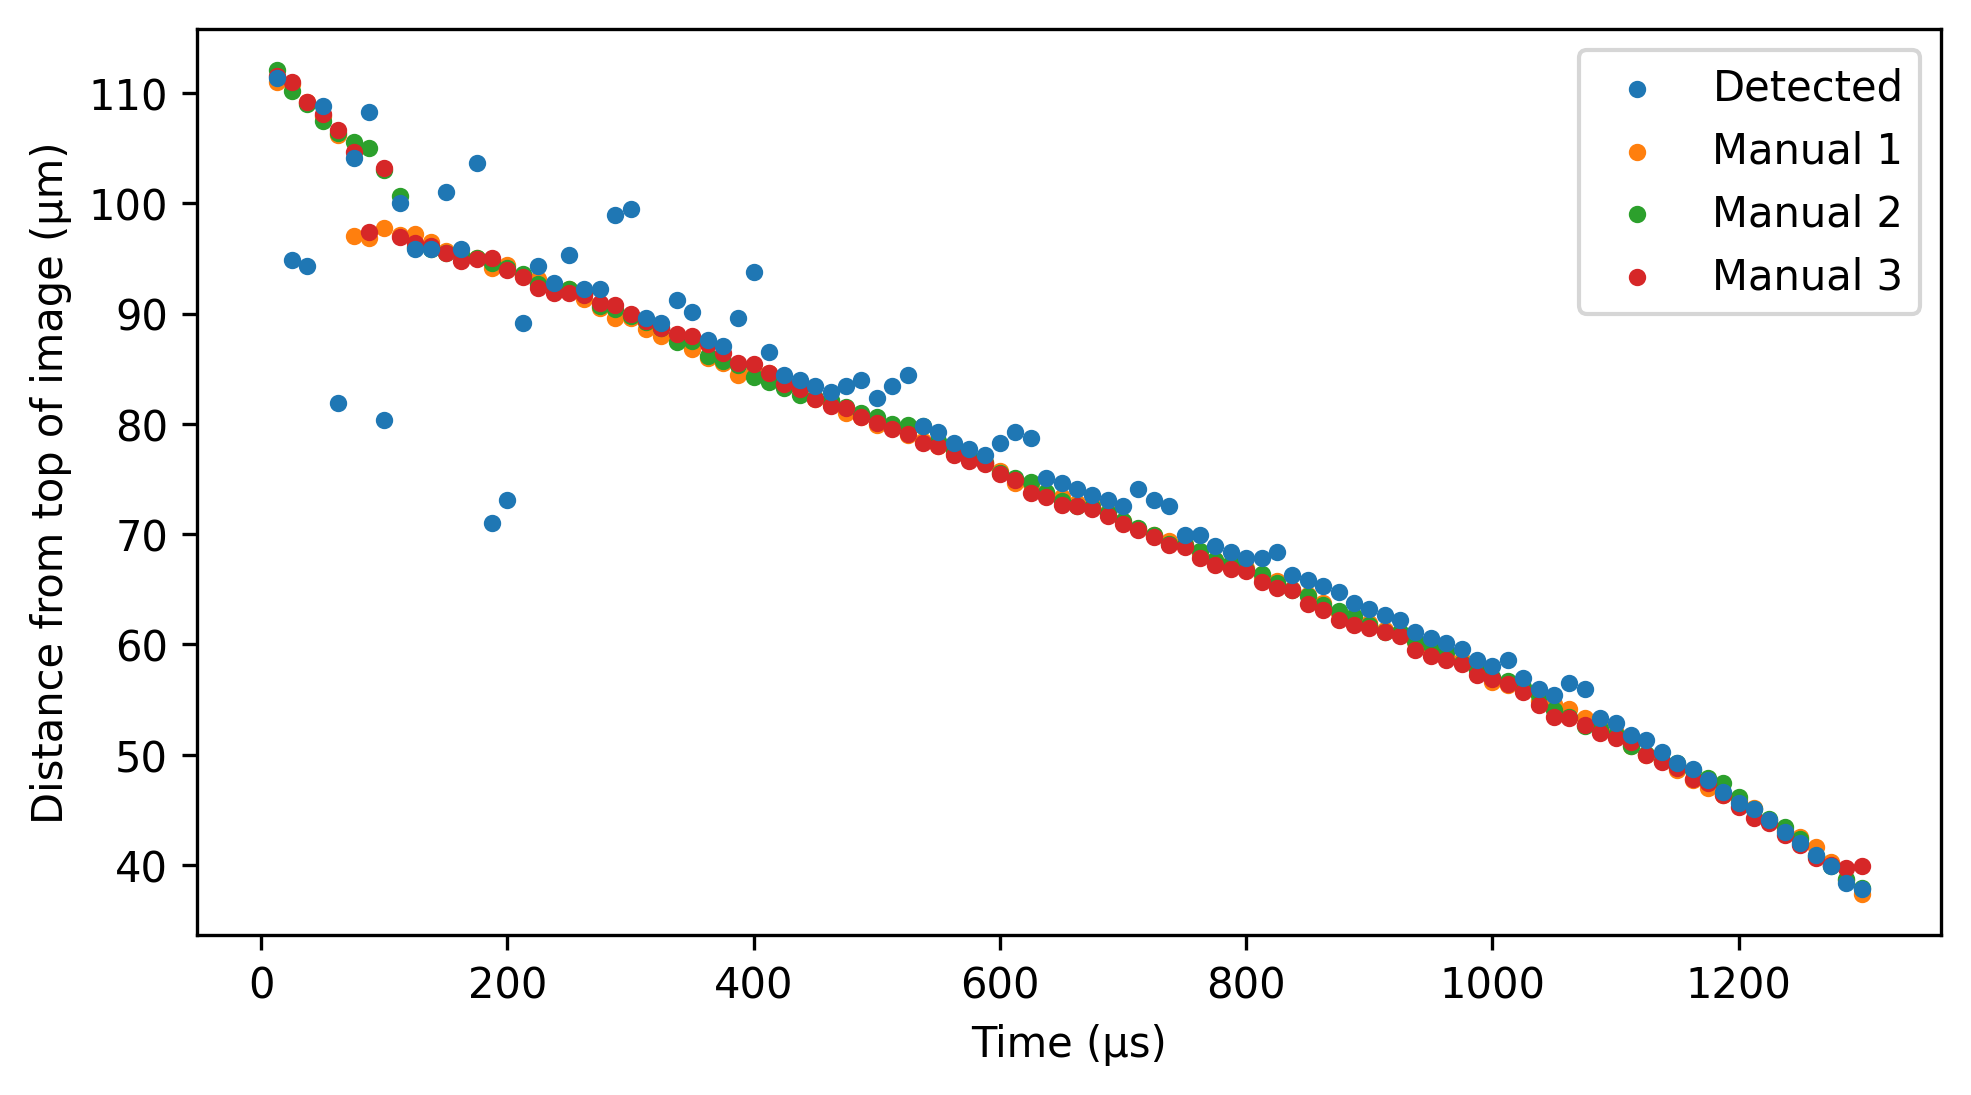
\includegraphics[width=0.75\textwidth]{figures/04/14-detected-vs-manual-3-12_shot01.png}
    \caption{
        \small\setstretch{1}
        Interfaces detected by the automated procedure (blue) compared with
        manually identified interfaces (orange, green, and red) for the
        208 W experiment. Interface location is defined by the distance from
        the bottom of the solid-liquid interface to top of the image,
        starting when the laser shuts off (t = 0 µs).
    }
    \label{fig/detected-aps-3}
\end{figure}

% -------------------------------------------------------------------------
\subsubsection{Rapid Solidification Results}
% -------------------------------------------------------------------------
The rapid solidification detection procedure and manual annotations are
performed on the data from three separate rapid solidification experiments.
For each of these
experiments, the mean and median velocity was calculated
for the major and minor axis lengths of the manually-measured and detected
ellipses.
In the first experiment, the average solidification velocities of the
three manually identified elliptical melt pools were calculated for the
major / minor axes as 2.164
m s\textsuperscript{-1} / 1.654 m s\textsuperscript{-1},
2.213 m s\textsuperscript{-1} / 1.690 m s\textsuperscript{-1}, and
2.172 m s\textsuperscript{-1} / 1.620 m s\textsuperscript{-1}. The
average major/minor axis velocities across all three measurements was
2.183 m s\textsuperscript{-1} / 1.655 m s\textsuperscript{-1} with medians of
2.167/1.580 m s\textsuperscript{-1}.

\begin{figure}[ht]
    \centering
    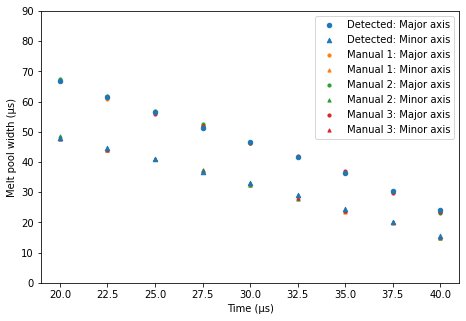
\includegraphics[width=0.75\textwidth]{figures/04/15-detected-vs-manual-03.png}
    \caption{
        \small\setstretch{1}
        Size of melt pools over time throughout the third rapid
        solidification experiment. The detected ellipses (blue) have a
        low deviation from the manually measured interfaces
        (orange, green, and red).
    }
    \label{fig/detected-dtem-1}
\end{figure}

In the second experiment, the average solidification velocities of the
three manually identified elliptical melt pools were calculated for the
major / minor axes as
2.268 m s\textsuperscript{-1} / 1.675 m s\textsuperscript{-1},
2.245 m s\textsuperscript{-1} / 1.773 m s\textsuperscript{-1}, and
2.234 m s\textsuperscript{-1} / 1.726 m s\textsuperscript{-1}. The
average major / minor axis velocities across all three measurements were
2.249 m s\textsuperscript{-1} / 1.725 m s\textsuperscript{-1} with medians
of 2.318/1.688 m s\textsuperscript{-1}.

\begin{figure}[ht]
    \centering
    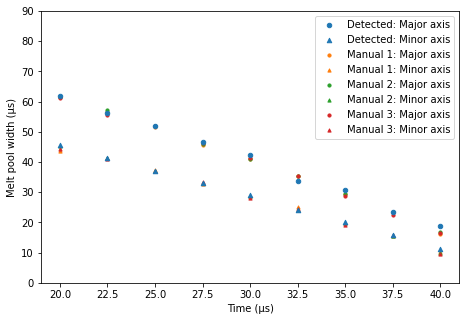
\includegraphics[width=0.75\textwidth]{figures/04/16-detected-vs-manual-04.png}
    \caption{
        \small\setstretch{1}
        Size of melt pools over time throughout the third rapid
        solidification experiment. The detected ellipses (blue) have a
        low deviation from the manually measured interfaces
        (orange, green, and red).
    }
    \label{fig/detected-dtem-2}
\end{figure}

In the third experiment, the average solidification velocities of the
three manually identified elliptical melt pools were calculated for the
major/minor axes as
2.665 m s\textsuperscript{-1} / 1.824 m s\textsuperscript{-1},
2.651 m s\textsuperscript{-1} / 1.871 m s\textsuperscript{-1}, and
2.602 m s\textsuperscript{-1} / 1.865 m s\textsuperscript{-1}. The
average major/minor axis velocities across all three measurements were
2.640 m s\textsuperscript{-1} / 1.853 m s\textsuperscript{-1} with medians
of 2.561 m s\textsuperscript{-1} / 1.856 m s\textsuperscript{-1}.

\begin{figure}[ht]
    \centering
    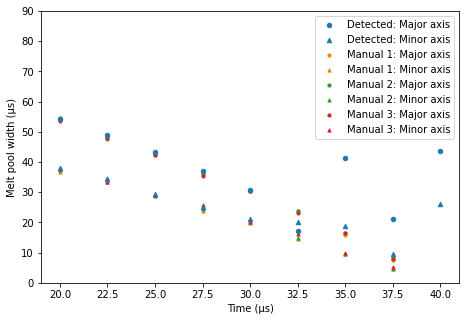
\includegraphics[width=0.75\textwidth]{figures/04/17-detected-vs-manual-09.png}
    \caption{
        \small\setstretch{1}
        Size of melt pools over time throughout the third rapid
        solidification experiment. The detected ellipses (blue) have a
        low deviation from the manually measured interfaces
        (orange, green, and red) until the end of the experiment.
    }
    \label{fig/detected-dtem-3}
\end{figure}

